\documentclass[russian,english]{llncs}
\usepackage[utf8]{inputenc}
\usepackage[T2A]{fontenc}
\usepackage[final]{graphicx}
\usepackage{epstopdf}
\usepackage[labelsep=period]{caption}
\usepackage[hyphens]{url}
\usepackage{amssymb,amsmath,mathrsfs}
\usepackage[russian,english]{babel}
%\usepackage{multicol}
\usepackage[ruled,vlined,linesnumbered,algo2e]{algorithm2e}
%\usepackage{algorithm}
%\usepackage[noend]{algorithmic}
\usepackage{color}
\usepackage{cmap}
\usepackage{array}
\usepackage{tikz}
\usepackage{pgfplots}
%\usepackage{verbatim}
\usepackage{standalone}

\tolerance=1000
\hbadness=5000
\newcommand{\const}{\mathrm{const}}
\newcommand{\tsum}{\mathop{\textstyle\sum}\limits}
\newcommand{\tprod}{\mathop{\textstyle\prod}\limits}
\newcommand{\cov}{\mathop{\rm cov}\limits}
\newcommand{\Dir}{\mathop{\rm Dir}\nolimits}
\newcommand{\norm}{\mathop{\rm norm}\limits}
\newcommand{\KL}{\mathop{\rm KL}\nolimits}
%\renewcommand{\geq}{\geqslant}
%\renewcommand{\leq}{\leqslant}
\newcommand{\eps}{\varepsilon}
\newcommand{\cond}{\mspace{3mu}{|}\mspace{3mu}}
\newcommand{\Loss}{\mathscr{L}}
\newcommand{\RR}{\mathbb{R}}
\newcommand{\cL}{\mathscr{L}}
\newcommand{\cP}{\mathscr{P}}
\newcommand{\kw}[1]{\textsf{#1}}
\SetKwFor{ForAll}{\textbf{for all}}{}{}

%... and these rows too.
\pgfplotsset{ every non boxed x axis/.append style={x axis line style=-},
     every non boxed y axis/.append style={y axis line style=-}}
\pgfplotsset{compat = 1.3}

\begin{document}
%%Analysis of Images, Social Networks, and Texts
\title{
    BigARTM: Open Source Library for
    Regularized Multimodal %Online Parallel Distributed
    Topic Modeling of Large Collections
}
\author{
    Konstantin Vorontsov\inst{1}
    \and
    Oleksandr Frei\inst{2}
    \and
    Murat Apishev\inst{3}
    \and
    Peter Romov\inst{4}
    \and
    Marina Dudarenko\inst{5}
}
\institute{\noindent
    Yandex,
    Moscow Institute of Physics and Technology,
    ~~\email{voron@forecsys.ru}
    \and
    Schlumberger Information Solutions,
    ~~\email{oleksandr.frei@gmail.com}
    \and
    Lomonosov Moscow State University,
    ~~\email{great-mel@yandex.ru}
    \and
    Yandex,
    Moscow Institute of Physics and Technology,
    ~~\email{peter@romov.ru}
    \and
    Lomonosov Moscow State University,
    ~~\email{m.dudarenko@gmail.com}
}

\maketitle

\begin{abstract}
Probabilistic topic modeling of text collections is a powerful tool for statistical text analysis.
In this paper we announce the \mbox{BigARTM} open source project (\texttt{http://bigartm.org}),
which provides the parallel online EM~algorithm 
for learning additively regularized multimodal topic models of large collections.
We~show that BigARTM outperforms other popular packages in quality, runtime and multicriteria functionality. 

\vspace{1em}
\textbf{Keywords:}
    probabilistic topic modeling,
    Probabilistic Latent Sematic Analysis,
    Latent Dirichlet Allocation,
    Additive Regularization of Topic Models,
    stochastic matrix factorization,
    EM~algorithm,
    BigARTM.
\end{abstract}

\section{Introduction}

Topic modeling is a~rapidly developing branch of statistical text analysis~\cite{blei12ptm}.
Probabilistic topic model (PTM) reveals a~hidden thematic structure of a~text collection.
It~defines each topic by a~discrete distribution over words,
and then describes each document with a~discrete distribution over topics.
Practical applications of topic models include many areas, such as
information retrieval for long-text queries,
%revealing research trends and research fronts,
classification, categorization, summarization of texts.
Modern literature on topic modeling offers hundreds of specialized models~\cite{daud10knowledge}.
Nevertheless,
most of these models are too difficult for practitioners
to quickly understand, adapt and embed into applications.
%This leads to a~common practice of tasting only the basic out-of-date models such as
%\emph{Probabilistic Latent Semantic Analysis}, PLSA~\cite{hofmann99plsi} and
%\emph{Latent Dirichlet Allocation}, LDA~\cite{blei03latent}.
Most practical inconveniences are rooted in Bayesian inference, 
which requires a~laborious mathematical work and prevents 
flexible unification, modification, selection, and combination of topic models.

In this paper we announce \textbf{the BigARTM open source project} for
regularized multimodal topic modeling of large collections,
\texttt{http://bigartm.org}.
The theory behind BigARTM is based on a non-Bayesian multicriteria approach~---
\emph{Additive Regularization of Topic Models}, ARTM~\cite{voron14dan-eng}.
Instead of building a~purely probabilistic generative model of text
we~regularize an ill-posed problem of stochastic matrix factorization
by~maximizing a~weighted sum of the log-likelihood and additional criteria.
Many known Bayesian topic models were revisited in terms of ARTM in~\cite{voron14mlj,voron14aist}.
Compared to the Bayesian approach,
ARTM makes it easier to design, infer and combine topic models,
thus reducing the barrier for entering into topic modeling research field.

%BigARTM source code is released under the New BSD License, which permits free commercial and non-commercial usage.
%The core of the library is written in C++ and is exposed via two equally rich APIs for C++ and Python.
%The library is cross-platform and can be built for Linux, Windows and OS X in both 32 and 64 bit configuration.
%
%In our experiments on Wikipedia corpus BigARTM performs better than Vowpal Wabbit LDA and Gensim libraries
%in terms of perplexity and runtime.
%Comparing to the other libraries BigARTM offers several additional features,
%such as regularization and multi-modal topic modeling.

In~section~\ref{sec:Multimodal}
we~introduce a~regularized multimodal topic model.
%In~section~\ref{sec:Online}
%we~generalize the~fast online algorithm~\cite{hoffman10online} to multimodal ARTM.
In~section~\ref{sec:BigARTM}
we~describe the parallel architecture of the BigARTM library.
In~section~\ref{sec:Experiments}
we~show that BigARTM performs better than Vowpal Wabbit LDA and Gensim libraries
in terms of perplexity and runtime on large Wikipedia corpus.
%In~section~\ref{sec:Conclusions}
%we~discuss advantages, limitations and open problems of BigARTM.

\section{Multimodal regularized topic model}
\label{sec:Multimodal}

%Matching Words and Pictures, MoM-LDA \cite{barnard03matching}
%\cite{virtanen12factorized}
%\cite{roller13multimodal}

Let
$D$ denote a finite set (collection) of texts and
$W^1$ denote a~finite set (vocabulary) of all terms from these texts.
A~document can contain not only words or~key phrases, but also terms of other modalities.
Each modality is defined by a finite set (vocabulary) of terms $W^m$, ${m=1,\dots,M}$.
Examples of not-word modalities are:
authors,
class or category labels,
date-time stamps,
links,
named entities,
objects on images,
users,
advertising banners,
etc.

Assume that
each term occurrence in each document refers to some latent topic from a~finite set of topics~$T$.
Text collection is considered to be a sample of triples
$(w_i,d_i,t_i)$,\; ${i=1,\dots,n}$,
drawn independently from a~discrete distribution $p(w,d,t)$ over the finite space $W\times D \times T$,
where ${W=W^1\sqcup\cdots\sqcup W^m}$ is a~disjoint union of the vocabularies across all modalities.
Terms~$w_i$ and documents~$d_i$ are observable variables,
while topics~$t_i$ are latent variables.

Following the idea of Correspondence LDA~\cite{blei03modeling}
and Dependency LDA~\cite{rubin12statistical}
we introduce a topic model for each modality:
\[
    p(w\cond d)
    = \sum_{t\in T} p(w\cond t)\: p(t\cond d)
    = \sum_{t\in T} \phi_{wt} \theta_{td},
    \quad
    d\in D,\; w\in W^m,\; m=1,\dots,M.
\]

The parameters
${\theta_{td}=p(t\cond d)}$ and ${\phi_{wt}=p(w\cond t)}$
form matrices
${\Theta = \bigl( \theta_{td} \bigr)_{T\times D}}$ of \emph{topic probabilities for the documents}, and
${\Phi^m = \bigl( \phi_{wt} \bigr)_{W^m\times T}}$ of \emph{term probabilities for the topics}.
The matrices $\Phi^m$, if stacked vertically, form a ${W\!\!\times\!T}$-matrix~$\Phi$.
Matrices $\Phi^m$ and~$\Theta$ are \emph{stochastic}
with vector-columns representing discrete distributions.
Usually~$|T|$ is much smaller than~$|D|$ and~$|W|$.

To learn parameters $\Phi^m$, $\Theta$ from the multimodal text collection
we maximize the log-likelihood for each $m$-th modality:
\[
    \cL_m (\Phi^m,\Theta) =
    \sum_{d\in D}\sum_{w\in W^m} n_{dw} \ln p(w\cond d)
    \to \max_{\Phi^m,\Theta},
\]
where
$n_{dw}$ is the number of occurrences of the term $w\in W^m$ in the document~$d$.
Following the ARTM approach,
we add a~regularization penalty term $R(\Phi,\Theta)$
and solve a constrained multicriteria optimization problem via scalarization:
\begin{gather}
\label{eq:multimodal}
    \sum_{m=1}^M \tau_m \cL_m (\Phi^m,\Theta)
    + R(\Phi,\Theta)
    \to \max_{\Phi,\Theta};
\\\label{eq:multimodal:norm}
    \sum_{w\in W^m}\!\!\! \phi_{wt} = 1,~
    \phi_{wt}\geq 0;
    \qquad
    \sum_{t\in T} \theta_{td} = 1,~
    \theta_{td}\geq 0.
\end{gather}

The local maximum $(\Phi,\Theta)$
of the problem~\eqref{eq:multimodal},~\eqref{eq:multimodal:norm}
satisfies the following system of equations
with auxiliary variables $p_{tdw} = p(t\cond d,w)$:
\begin{align}
    \label{eq:Estep}
    p_{tdw} &= \norm_{t\in T} \bigl(\phi_{wt}\theta_{td}\bigr);
\\
    \label{eq:Mstep:phi}
    \phi_{wt} &= \norm_{w\in W^m}
        \biggl(
            n_{wt} + \phi_{wt} \frac{\partial R}{\partial \phi_{wt}}
        \biggr);
    \quad
    n_{wt} = \sum_{d\in D} \tau_{m(w)} n_{dw} p_{tdw};
\\
    \label{eq:Mstep:theta}
    \theta_{td} &= \norm_{t\in T}
        \biggl(
            n_{td} + \theta_{td} \frac{\partial R}{\partial \theta_{td}}
        \biggr);
    \quad
    n_{td} = \sum_{w\in d} \tau_{m(w)} n_{dw} p_{tdw};
        %\sum_{m=1}^M \tau_m \!\!\sum_{w\in W^m}\!\!\! n_{dw} p_{tdw};
\end{align}
where operator
$\norm_{t\in T} x_t = \frac{\max\{x_t,0\}}{\sum\limits_{s\in T} \max\{x_s,0\}}$
transforms a~vector $(x_t)_{t\in T}$ to a~discrete distribution;
$m(w)$~is the modality of the term~$w$, so that $w\in W^{m(w)}$.

The system of equations \eqref{eq:Estep}--\eqref{eq:Mstep:theta}
follows from Karush--Kuhn--Tucker conditions.
Solving it by the simple-iteration method is equivalent to the EM~algorithm,
which repeats 
E-step \eqref{eq:Estep} and
M-step \eqref{eq:Mstep:phi}--\eqref{eq:Mstep:theta}
in a~loop.
For single modality (${M=1}$) it corresponds to the regularized EM~algorithm~\cite{voron14dan-eng}.
With no regularization (${R=0}$) it~corresponds to 
\emph{Probabilistic Latent Semantic Analysis}, PLSA~\cite{hofmann99plsi}.
Many Bayesian topic models 
including \emph{Latent Dirichlet Allocation}, LDA~\cite{blei03latent},
can be considered as special cases of ARTM with different regularizers~$R$~\cite{voron14mlj,voron14aist}.

The most important feature of ARTM is that it allows to combine regularizers additively:
$R(\Phi,\Theta) = \sum_{i=1}^r \lambda_i R_i(\Phi,\Theta)$,
which leads to an easy modification of the M-step.
BigARTM provides a~build-in user extendable library of~regularizers.

\section{BigARTM architecture}
\label{sec:BigARTM}

BigARTM implements a~fast online EM~algorithm
similar to the Online LDA~\cite{hoffman10online}.
We~split the collection into batches,
and run EM iterations so that
each document vector $\theta_d$ is~iterated until convergence at a~constant matrix~$\Phi$.
\mbox{Matrix}~$\Phi$ is updated after all documents from the batch are processed.
For a~large collection
matrix~$\Phi$ often stabilizes after small initial part of the collection.
Therefore a~single pass through the collection might be sufficient to learn a~topic model.
%The second pass may be needed for the initial part of the collection.

%\mbox{Matrix}~$\Phi$ can be updated after every batch or less frequently
%(for instance if it takes long time to evaluate all regularizers).
%This flexibility is important for concurrent implementation of the algorithm,
%where multiple batches are processed in parallel.
%In~this case synchronization can be triggered when a fixed number of documents had been processed since the last synchronization.
%
%The online reorganization of the EM iterations
%is not necessarily associated with Bayesian inference used in~\cite{hoffman10online}.
%Different topic models, from PLSA to multimodal and regularized models,
%can be learned by the above online EM algorithm.

BigARTM processes a~large collection without loading it entirely into the memory.
This is achieved by storing each batch in a separate file on disk,
and loading a limited number of batches into the main memory at any given time.

To split collection into batches and process them concurrently is a common approach,
introduced in AD-LDA algorithm \cite{newman09distributed}, and
then further developed in PLDA \cite{wang09plda} and PLDA{+} \cite{liu11plda} algorithms.
These algorithms require all concurrent workers to become idle before an update of the $\Phi$ matrix.
Such synchronization step adds a large overhead in the online algorithm where $\Phi$ matrix is updated multiple times on each iteration.
An alternative architecture without the synchronization step is described in \cite{smola10architecture},
however it mostly targets a distributed cluster environment.
In our work we develop an efficient single-node architecture where all workers benefit from the shared memory space.

The BigARTM out-of-core implementation avoids storing full $\Theta$ matrix in the memory
by calculating $\theta_{td}$ on the fly during a~batch processing.
The inference of $\theta_{td}$ is executed in parallel in such a way that many batches are processed concurrently,
however each batch is processed by simple single-threaded code.
This 
%makes it easy to optimize this performance-critical routine,
%and at the same time
gives almost linear speedup with the number of processors.

Processing each batch results in an $n_{wt}$ increment that has to be applied to the $\Phi$~matrix.
We merge $n_{wt}$ in a background, and asynchronously build a new $\Phi$~matrix.
This doubles the memory usage, but enables BigARTM to update $\Phi$~matrix without pausing all batch processing threads.
%As a result, BigARTM avoids this costly synchronization step, which is important for online algorithm
%where $\Phi$ matrix is updated multiple times on each iteration.
All processor threads share the same $\Phi$ matrix,
which means that memory usage stays at constant level regardless of how many cores are used for computation.

%Using memory for two copies of the $\Phi$ matrix in our opinion gives a reasonable usage balance between memory and CPU resources.
%An~alternative solution with only one $\Phi$ matrix is also possible, but it would require a heavy usage of atomic CPU instructions.
%Such operations are very efficient, but still come at a considerable synchronization cost%
%\footnote{\url{http://stackoverflow.com/questions/2538070/atomic-operation-cost}},
%and using them for all reads and writes of the $\Phi$ matrix would cause a significant performance degradation for merger and processor threads.
%Besides, an arbitrary overlap between reads and writes of the $\Phi$ matrix eliminates any possibility of producing a deterministic result.
%The design with two copies of the $\Phi$ matrix gives much more control over this
%and in certain cases allows BigARTM to behave in a fully deterministic way.

BigARTM uses dense single-precision matrices to represent $\Phi$ and~$\Theta$.
Together with the $\Phi$ matrix we store a global dictionary of all terms ${w \in W}$.
%This dictionary is implemented as $\kw{std::unordered\_map}$ that maps a string representation of ${w \in W}$
%into its integer index in the $\Phi$ matrix.
This dictionary can be extended automatically as more and more batches came through the system.
To~achieve this each batch contains a local dictionary, listing all terms that occur in the batch.
The $n_{dw}$ elements of the batch are stored as a~sparse CSR matrix (Compressed Sparse Raw format),
where rows correspond to documents from the batch, and terms run over the~local batch dictionary.

%For performance reasons $\Phi$ matrix is stored in column-major order, and $\Theta$ in row-major order.
%This layout ensures that $\sum_t \phi_{wt} \theta_{td}$ sum runs on contiguous memory blocks.
%We also take special precautions to avoid performance issues with denormalized numbers%
%\footnote{\url{http://en.wikipedia.org/wiki/Denormal_number#Performance_issues}}.
%%http://stackoverflow.com/questions/9314534/why-does-changing-0-1f-to-0-slow-down-performance-by-10x

The core of the library is written in C++ and is exposed via two equally rich APIs for C++ and Python
(Java wrapper is planned in the near future).
%BigARTM has built-in libraries of regularizers and quality measures that can be extended through project recompilation.
To input and output complex data structures the API uses Google Protocol Buffers.
This approach makes it easy to integrate BigARTM into any research or production environment.
The library is cross-platform and can be built for Linux, Windows and OS X in both 32 and 64 bit configuration.

BigARTM source code is released under the New BSD License, which permits free commercial and non-commercial usage.

\section{Experiments}
\label{sec:Experiments}

In the first experiment, 
we evaluate the \mbox{BigARTM} performance against two popular software packages~---
Gensim~\cite{rehurek10software}
%\footnote{\url{http://radimrehurek.com/gensim/}}
and Vowpal Wabbit (VW)%
\footnote{\url{https://github.com/JohnLangford/vowpal_wabbit/}}
on a~collection of 3.7~million articles from the English Wikipedia%
\footnote{\url{http://dumps.wikimedia.org/enwiki/20141208/}}.
%The conversion to bag-of-words was done with $\kw{gensim.make\_wikicorpus}$ script%
%\footnote{\url{https://github.com/piskvorky/gensim/tree/develop/gensim/scripts/}},
%which excludes pages shorter than $50$~words.
Both use the Online Variational Bayes LDA \cite{hoffman10online}.
\mbox{VW.LDA} is one of the fastest single-threaded implementation in~C++.
Gensim has two LDA implementations:
LdaModel processes all batches sequentially,
%and the concurrency happens entirely within NumPy library;
LdaMulticore processes several batches concurrently similar to \mbox{BigARTM}.
The dictionary is formed by $|W| = 100\,000$ most frequent words.
Each run performs one pass over the Wikipedia corpus and produces a~model with $|T|=100$ topics.
Batch size is $10\,000$ documents.
The perplexity measure is defined as
$\mathcal{P}(D, p) = \exp \bigl( - \frac{1}{n} \sum_{d,w} n_{dw} \ln p(w \cond d) \bigr)$.
Table\;\ref{tab:libraries_comparison} compares the performance results
for an Intel-based CPU with 16 physical cores with hyper-threading.
Fig.\;\ref{fig:bigartm_speedup} shows BigARTM speedup and memory consumption depending on the number of CPU threads
for Amazon AWS~c3.8xlarge with 32~virtual cores.

\begin{table}[t]
	\caption{
        The comparison of BigARTM with VW.LDA and Gensim.
        \emph{Train} is the time for model training,
        \emph{inference} is the time for calculation of $\theta_d$ of $100\,000$ held-out documents,
        \emph{perplexity} is calculated on held-out documents.
    }
	\label{tab:libraries_comparison}
    \centering\tabcolsep=4.3pt
	\begin{tabular}[t]{l|c|rrr}
	\hline
	library & procs & train & inference & perplexity \\
	\hline
	BigARTM & 1 & 35 min & 72 sec & 4000 \\
	LdaModel & 1 & 369 min & 395 sec & 4161  \\
	VW.LDA & 1 & 73 min & 120 sec & 4108 \\
	\hline
	BigARTM & 4 & 9 min & 20 sec & 4061  \\
	LdaMulticore & 4 & 60 min & 222 sec & 4111  \\	
	\hline
	BigARTM & 8 & 4.5 min & 14 sec & 4304  \\
	LdaMulticore & 8 & 57 min & 224 sec & 4455 \\
	\hline
	\end{tabular}
\end{table}

\begin{figure}[t]
	\centering
	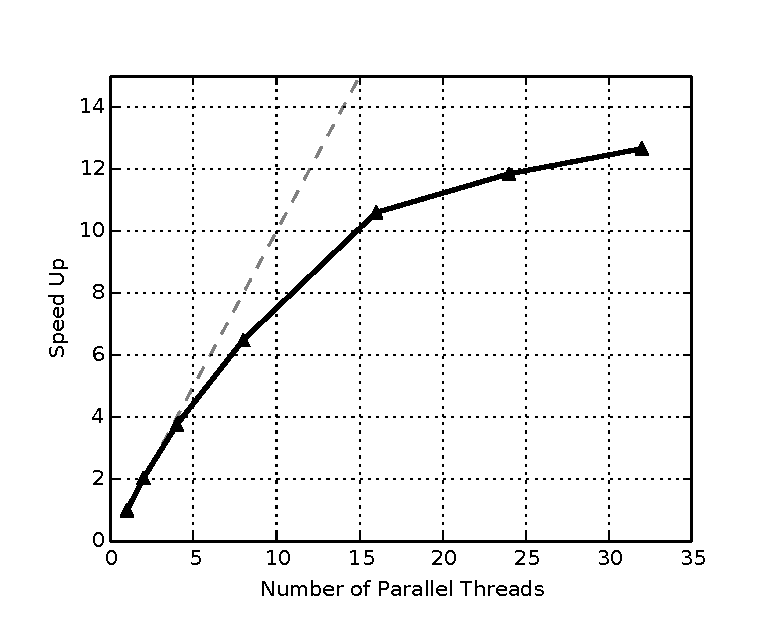
\includegraphics[height=35mm]{bigartm_speedup.eps}
	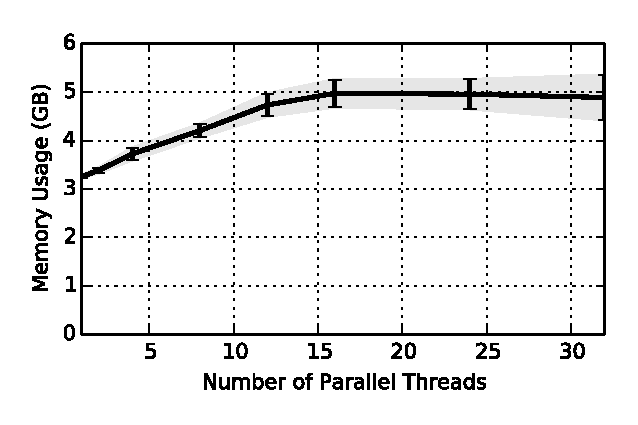
\includegraphics[height=35mm]{bigartm_memory.eps}
	\caption{Running BigARTM in parallel: speed up (left) and memory usage (right)}
	\label{fig:bigartm_speedup}
\end{figure}

In~the second experiment, 
we combine three regularizers from the BigARTM built-in library:
$\phi_{t}$~sparsing,
$\theta_{d}$~sparsing, and
$\phi_{t}$~decorrelation.
This combination has improved several quality measures without significant loss of perplexity
in~previous experiments with offline implementation of ARTM~\cite{voron14aist}.
Table \ref{tab:model_comparison} shows that this remains true for the BigARTM implementation.
Figure \ref{fig:comparison_plot} shows the convergence of quality measures on the number of processed documents.

\begin{table}[t]
    \caption{Comparison of LDA and ARTM models.
        Quality measures:
        $\mathcal{P}_{10k}$, $\mathcal{P}_{100k}$ --- perplexity on 10K and 100K hold-out document sets,
        $\mathcal{S}_{\Phi}$, $\mathcal{S}_{\Theta}$ --- sparsity of $\Phi$ and $\Theta$ matrices (in~\%),
        $\mathcal{K}_{p}$, $\mathcal{K}_{c}$ --- average topic purity and contrast respectively.}
    \label{tab:model_comparison}
    \centering\vskip-2ex\tabcolsep=8pt
    \begin{tabular}[t]{l|rrrrrrr}
    \hline
    Model & $\mathcal{P}_{10k}$ & $\mathcal{P}_{100k}$ &  $\mathcal{S}_{\Phi}$ & $\mathcal{S}_{\Theta}$ &  $\mathcal{K}_{p}$ &  $\mathcal{K}_{c}$ \\
    \hline
        LDA    & 3436 & 3801 & 0.0  & 0.0  & 0.533 & 0.507 \\
        ARTM   & 3577 & 3947 & 96.3 & 80.9 & 0.785 & 0.731 \\
    \hline
    \end{tabular}
\end{table}

\begin{figure}[t]
    \centering
    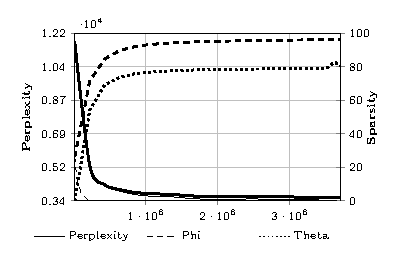
\includegraphics[width=60mm]{plot_perplexity_sparsity.eps}\hfill
    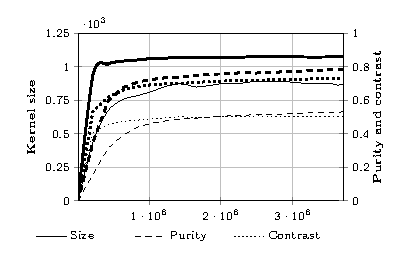
\includegraphics[width=60mm]{plot_kernel.eps}
\caption{Comparison of LDA (thin) and ARTM (bold) models. 
    The number of processed documents is shown along the X~axis.
    The left chart shows perplexity and sparsity of $\Phi$, $\Theta$ matrices, and
    the right chart shows average lexical kernel measures.
}
\label{fig:comparison_plot}
\end{figure}

In the third experiment,
we show how BigARTM works with multimodal datasets. 
We~prepared a text corpus containing 216\,175~pairs of English and Russian Wikipedia articles with mutual interwiki links.
We~represent each linked pair of articles
as a~single document with~two modalities, one modality for each language.
The combined dictionary contains $|W|=196\,749$ words (43\% Russian, 57\% English).
We build a~model with $|T|=400$ topics.
An~independent assessor successfully interpreted all except four topics.
Table \ref{tab:top10words} shows top 10~words for four randomly selected topics.
Top words in these topics are clearly consistent between Russian and English languages.

\begin{table}[t!]
	\caption{
        Top 10 words with $p(w\cond t)$ probabilities (in~\%) from two-language topic model,
        based on Russian and English Wikipedia articles with mutual interlanguage links.}
	\label{tab:top10words}
	\centering\tabcolsep=3pt%\small
	\footnotesize
    \begin{tabular}{|lr|lr||lr|lr|}	
    	\hline
    	\multicolumn{4}{|c||}{\textbf{Topic~68}} & \multicolumn{4}{c|}{\textbf{Topic~79}\rule{0pt}{3ex}} \\
    	\hline
    	research & 4.56 & институт & 6.03 & goals & 4.48 & матч & 6.02 \\
    	technology & 3.14 & университет & 3.35 & league & 3.99 & игрок & 5.56 \\
    	engineering & 2.63 & программа & 3.17 & club & 3.76 &  сборная & 4.51 \\
    	institute & 2.37 & учебный & 2.75 & season & 3.49 & фк & 3.25 \\
    	science & 1.97 & технический & 2.70 & scored & 2.72 & против & 3.20 \\
    	program & 1.60 & технология & 2.30 & cup & 2.57 & клуб & 3.14 \\
    	education & 1.44 & научный & 1.76 & goal & 2.48 & футболист & 2.67 \\
    	campus & 1.43 & исследование & 1.67 & apps & 1.74 & гол & 2.65 \\
    	management & 1.38 & наука & 1.64 & debut & 1.69 & забивать & 2.53 \\
    	programs & 1.36 & образование & 1.47 & match & 1.67 & команда & 2.14 \\
    	\hline
    	\multicolumn{4}{|c||}{\textbf{Topic~88}} &     \multicolumn{4}{c|}{\textbf{Topic~251}\rule{0pt}{3ex}}  \\
    	\hline
        opera & 7.36 & опера & 7.82 & windows & 8.00 & windows & 6.05 \\
    	conductor & 1.69 & оперный & 3.13 & microsoft & 4.03 & microsoft & 3.76 \\
    	orchestra & 1.14 & дирижер & 2.82 & server & 2.93 & версия & 1.86 \\
    	wagner & 0.97 & певец & 1.65 & software & 1.38 & приложение & 1.86 \\
    	soprano & 0.78 & певица & 1.51 & user & 1.03 & сервер & 1.63 \\
    	performance & 0.78 & театр & 1.14 & security & 0.92 & server & 1.54 \\
    	mozart & 0.74 & партия & 1.05 & mitchell & 0.82 & программный & 1.08 \\
    	sang & 0.70 & сопрано & 0.97 & oracle & 0.82 &  пользователь & 1.04 \\
    	singing & 0.69 & вагнер & 0.90 & enterprise & 0.78 & обеспечение & 1.02 \\
    	operas & 0.68 & оркестр & 0.82 & users & 0.78 & система & 0.96 \\
    	\hline
	\end{tabular}
\end{table}


%There are many efficient LDA implementations for single node processing.
%In this section we discuss Vowpal Wabbit LDA \cite{vwlda} and Gensim \cite{gensim} as most popular ones.
%At first we review their technical and algorithmic features and compare them with solutions applied to our library.
%In addition we explain the reasons why we refused to integrate ARTM into these implementations.
%Then we compare the results of experiments on these libraries and BigARTM.
%
%\paragraph{Vowpal Wabbit LDA.} LDA in Vowpal Wabbit is online, as other algorithms in this library.
%It bases on Online Variational Bayes LDA described by Matthew Hoffman in \cite{hoffman10online}.
%Online VB LDA in Vowpal Wabbit supports single-threaded documents processing, it's neither a multi-core nor distributed.
%Nevertheless, effective implementation in C++ without STL and good scalability of the algorithm
%made VW.LDA one of the fastest tools for topic modeling within single computing node.
%However, it's not very comfortable: Vowpal Wabbit LDA doesn't have user API and launches from CLI.
%This implies the limitations of possibilities to tune the parameters of topic model and to control its quality.
%
%Online algorithm and C++ usage are the common features of BigARTM and VW.LDA
%\footnote{But we also use STL ? Boost libraries}. Also both of libraries are cross-platform.
%But there are more differences than similarities. BigARTM accelerates processing by using multithreaded computing.
%Library capabilities and user API are much richer. API allows to tune almost all phases of algorithm.
%At the same time, it's also possible to use library from CLI as in VW.LDA, if necessary.
%
%\paragraph{Gensim.} Cross-platform and written on Python, library Gensim has two different LDA implementations.
%The first one is LdaModel, it's almost a clone of Online VB LDA.
%The high performance of data processing is achieved through the usage of NumPy library, built over low-level BLAS library
%\footnote{Intel MKL, ATLAS etc.}. The second implementation is LdaMulticore.
%It also bases on Online VB LDA, but supports multi-core processing. LdaMulticore creates a workflow per core,
%which processes it's own part of documents. In addition, it creates a general aggregating stream, that merges
%asynchronously the results, recieved from workflows. In this way, LdaModel uses several cores to process one batch of documents,
%and in LdaMulticore each core processes it's own batch. Gensim has a comfortable enough user interface.
%Moreover, it has a capability to find topic distributions for new documents using pre-built topic model.
%
%BigARTM and Gensim.LdaMulticore proceed multithreaded data processing in the same way.
%BigARTM also can find topic distributions for new documents. But our library supports multimodal models.
%And it's more productive. In the following experiments we show,
%that BigARTM's scalability is higher, than LdaMulticore's one.
%
%\paragraph{Motivation.} BigARTM's idea is to create a versatile tool for topic modeling that meets several criteria:
%
%\begin{itemize}
%	\item Online data processing.
%	\item ARTM support with possibility to add new regularizers and functionals of quality.
%	\item Permanent monitoring of topic model during learning.
%	\item A capability to be integrated in other programming languages.
%	\item Efficient parallel data processing.
%	\item Rich and flexible user API.
%	\item Cross-platform.
%\end{itemize}
%Some of this conditions exclude the possibility of using VW.LDA or Gensim as the base of ARTM.
%Vowpal Wabbit is a common library of online algorithms, which contain LDA as one of the working modes.
%It's impossible to control the state of the model or to influence it during the learning process.
%As we noted above, there's no user API in VW.LDA.
%In addtition, the source code of the library is difficult for modification and support.
%
%The key reason we refused to implement ARTM in Gensim is that it's written on Python.
%This language doesn't provide the possibility to be integrated into other languages easy.
%And C++ does. Moreover, we consider Gensim.LdaMulticore to be not very efficient. This question is discussed below.
%
%BigARTM satisfies all of the given criteria. It's effective, easily extensible due to the plug-ins,
%supports user interfaces for different languages. As we noted above, the library can learn several topic models simultaneously,
%apply different regularization strategies. Also it allows to correct parameters
%of the regularizers and models during the learning process and unload any intermediate and final information about the models.

\section{Conclusions}
\label{sec:Conclusions}

\mbox{BigARTM} in an open source project for parallel online topic modeling of large text collections.
It~provides a~high flexibility for various applications due to
multimodality and additive combinations of regularizers.
%\mbox{BigARTM} architecture has a~rich potential.
%Current components can be reused in a~distributed solution that runs on cluster.
%Further improvement of single-node can be achieved by offloading batch processing into GPU.

\medskip
\paragraph{Acknowledgements.}
    The work was supported by~the Russian Foundation for Basic Research grants 14-07-00847, 14-07-00908, 14-07-31176
    and by~Skolkovo Institute of Science and Technology (project 081-R).


%%%%%%%%%%%%%%%%%%%%%%%%%%%%%%%%%%%%%%%%%%%%%%%%%%%%%%%%%%%%%%%%%%%%%%%%%%%%
%\bibliographystyle{splncs03}
%\bibliography{MachLearn}

\begin{thebibliography}{10}
%\providecommand{\url}[1]{\texttt{#1}}
%\providecommand{\urlprefix}{URL }

\bibitem{blei12ptm}
Blei, D.M.: Probabilistic topic models. Communications of the ACM  55(4),
  77--84 (2012)

\bibitem{blei03modeling}
Blei, D.M., Jordan, M.I.: Modeling annotated data. In: Proceedings of the 26th
  Annual International ACM SIGIR Conference on Research and Development in
  Informaion Retrieval. pp. 127--134. ACM, New York, NY, USA (2003)

\bibitem{blei03latent}
Blei, D.M., Ng, A.Y., Jordan, M.I.: Latent {Dirichlet} allocation. Journal of
  Machine Learning Research  3,  993--1022 (2003)

\bibitem{daud10knowledge}
Daud, A., Li, J., Zhou, L., Muhammad, F.: Knowledge discovery through directed
  probabilistic topic models: a survey. Frontiers of Computer Science in China
  4(2),  280--301 (2010)

\bibitem{hoffman10online}
Hoffman, M.D., Blei, D.M., Bach, F.R.: Online learning for latent Dirichlet
  allocation. In: NIPS. pp. 856--864. Curran Associates, Inc. (2010)

\bibitem{hofmann99plsi}
Hofmann, T.: Probabilistic latent semantic indexing. In: Proceedings of the
  22nd annual international ACM SIGIR Conference on Research and Development in
  Information Retrieval. pp. 50--57. ACM, New York, NY, USA (1999)

\bibitem{liu11plda}
Liu, Z., Zhang, Y., Chang, E.Y., Sun, M.: {PLDA+:} parallel latent {D}irichlet
  allocation with data placement and pipeline processing. ACM Trans. Intell.
  Syst. Technol.  2(3),  26:1--26:18 (May 2011)

\bibitem{newman09distributed}
Newman, D., Asuncion, A., Smyth, P., Welling, M.: Distributed algorithms for
  topic models. J. Mach. Learn. Res.  10,  1801--1828 (Dec 2009)

\bibitem{rubin12statistical}
Rubin, T.N., Chambers, A., Smyth, P., Steyvers, M.: 
  Statistical topic models for multi-label document classification. 
  Machine Learning  88(1--2),  157--208
  (2012)

\bibitem{smola10architecture}
Smola, A., Narayanamurthy, S.: An architecture for parallel topic models. 
    Proc. VLDB Endow.  3(1--2),  703--710 (Sep 2010)

\bibitem{voron14dan-eng}
Vorontsov, K.V.: Additive regularization for topic models of text collections.
  Doklady Mathematics  89(3),  301--304 (2014)

\bibitem{voron14mlj}
Vorontsov, K.V., Potapenko, A.A.: Additive regularization of topic models.
  Machine Learning, Special Issue on Data Analysis and Intelligent Optimization
   (2014)

\bibitem{voron14aist}
Vorontsov, K.V., Potapenko, A.A.: Tutorial on probabilistic topic modeling:
  Additive regularization for stochastic matrix factorization. In: AIST'2014,
  Analysis of Images, Social networks and Texts. vol. 436, pp. 29--46. 
  Springer, CCIS (2014)

\bibitem{rehurek10software}
\v{R}eh\r{u}\v{r}ek, R., Sojka, P.: Software framework for topic modelling with
  large corpora. In: Proceedings of the {LREC} 2010 Workshop on New Challenges
  for {NLP} Frameworks. pp. 45--50. {ELRA}, Valletta, Malta (May 2010)

\bibitem{wang09plda}
Wang, Y., Bai, H., Stanton, M., Chen, W.Y., Chang, E.Y.: {PLDA}: Parallel
  latent {D}irichlet allocation for large-scale applications. In: Proceedings
  of the 5th International Conference on Algorithmic Aspects in Information and
  Management. pp. 301--314. AAIM '09, Springer-Verlag, Berlin, Heidelberg
  (2009)

\end{thebibliography}
%%%%%%%%%%%%%%%%%%%%%%%%%%%%%%%%%%%%%%%%%%%%%%%%%%%%%%%%%%%%%%%%%%%%%%%%%%%%

%%%\newpage
%%%\section*{Appendix A}
%%%
%%%Consider the system of equations \eqref{eq:Estep}--\eqref{eq:Mstep:theta}.
%%%
%%%Topic~$t$ is called \emph{regular} for the modality~$m$
%%%if ${n_{wt} + \phi_{wt} \frac{\partial R}{\partial \phi_{wt}} > 0}$
%%%for at least one term ${w\in W^m}$.
%%%If~the~reverse inequality holds for all ${w\in W^m}$ then
%%%topic~$t$ is called \emph{irregular}.
%%%
%%%Document~$d$ is called \emph{regular}
%%%if ${n_{td} + \theta_{td} \frac{\partial R}{\partial \theta_{td}} > 0}$
%%%for at least one topic ${t\in T}$.
%%%If~the reverse inequality holds for all ${t\in T}$ then
%%%document~$d$ is called \emph{irregular}.
%%%
%%%\begin{theorem}
%%%\label{th:multimodal}
%%%    If the function $R(\Phi,\Theta)$ is continuously differentiable
%%%    and $(\Phi,\Theta)$ is the local maximum
%%%    of the problem~\eqref{eq:multimodal},~\eqref{eq:multimodal:norm}
%%%    then for any regular topic-modality pair $(t,m)$ and any regular document~$d$
%%%    the system of equations \eqref{eq:Estep}--\eqref{eq:Mstep:theta} holds.
%%%\end{theorem}
%%%
%%%\begin{note}
%%%    If a~topic~$t$ is irregular
%%%    then the $t$-th vector-column in matrix~$\Phi^m$ equals zero
%%%    and can not represent a~discrete distribution.
%%%    This means that topic~$t$ for the modality~$m$ must be excluded from the model.
%%%    This mechanism is useful for irrelevant topics elimination and determining the number of topics.
%%%\end{note}
%%%\begin{note}
%%%    If a~documents~$d$ is irregular
%%%    then the $d$-th vector-column in matrix~$\Theta$ equals zero
%%%    and can not represent a~discrete distribution.
%%%    This means that document~$d$ must be excluded from the model.
%%%    For example, a~document may be too short or irrelevant to the given collection.
%%%\end{note}
%%%
%%%\begin{proof}
%%%    For the local minimum $\Phi^m,\Theta$
%%%    of the problem~\eqref{eq:multimodal},~\eqref{eq:multimodal:norm}
%%%    the Karush--Kuhn--Tucker (KKT) conditions can be written as follows:
%%%    %(conditions with respect to $\theta_{td}$ are analogous):
%%%    \begin{gather*}
%%%        \sum_{d} n_{dw} \frac{\theta_{td}}{p(w\cond d)} + \frac{\partial R}{\partial \phi_{wt}}
%%%        = \lambda_t - \lambda_{wt};
%%%        \quad
%%%        \lambda_{wt}\geq 0;
%%%        \quad
%%%        \lambda_{wt}\phi_{wt} = 0;
%%%    \\
%%%        \sum_{m} \tau_m \!\!\sum_{w\in W^m}\!\! n_{dw} \frac{\phi_{wt}}{p(w\cond d)} + \frac{\partial R}{\partial \theta_{td}}
%%%        = \mu_d - \mu_{td};
%%%        \quad
%%%        \mu_{td}\geq 0;
%%%        \quad
%%%        \mu_{td}\theta_{td} = 0;
%%%    \end{gather*}
%%%    where $\lambda_t$, $\lambda_{wt}$, $\mu_d$, $\mu_{td}$
%%%    are KKT multipliers for normalization and nonnegativity constrains.
%%%
%%%    Let us multiply
%%%    both sides of the first equation by~$\phi_{wt}$,
%%%    both sides of the second equation by~$\theta_{td}$,
%%%    and reveal the auxiliary variable~$p_{tdw}$ from~\eqref{eq:Estep}
%%%    in~the~left-hand side of both equations.
%%%    Then we sum
%%%    the right-hand side of the first equation over~$d$,
%%%    the right-hand side of the second equation over~$t$:
%%%    \begin{gather*}
%%%        \phi_{wt} \lambda_t
%%%        =
%%%        \sum_{d}
%%%        n_{dw} \frac{\phi_{wt}\theta_{td}}{p(w\cond d)}
%%%        + \phi_{wt} \frac{\partial R}{\partial \phi_{wt}}
%%%        =
%%%        n_{wt} + \phi_{wt} \frac{\partial R}{\partial \phi_{wt}};
%%%    \\
%%%        \theta_{td} \mu_{d}
%%%        =
%%%        \sum_{m} \tau_m \!\!\sum_{w\in W^m}\!\!
%%%        n_{dw} \frac{\phi_{wt}\theta_{td}}{p(w\cond d)}
%%%        + \theta_{td} \frac{\partial R}{\partial \theta_{td}}
%%%        =
%%%        n_{td} + \theta_{td} \frac{\partial R}{\partial \theta_{td}}.
%%%    \end{gather*}
%%%
%%%    An~assumption that $\lambda_t\leq 0$ contradicts the regularity condition for the $(t,m)$ pair.
%%%    Then ${\lambda_t>0}$.
%%%    Either ${\phi_{wt}= 0}$ or both sides of the first equation are positive.
%%%    Combining these two cases in one formula, we write:
%%%    \begin{equation}
%%%    \label{eq:in-theorem-1:phi}
%%%        \phi_{wt} \lambda_t
%%%        =
%%%        \max\biggl\{
%%%        n_{wt} + \phi_{wt} \frac{\partial R}{\partial \phi_{wt}}, 0
%%%        \biggr\}.
%%%    \end{equation}
%%%    Analogously,
%%%    an~assumption that $\mu_d\leq 0$ contradicts the regularity condition for the document~$d$.
%%%    Then ${\mu_d>0}$.
%%%    Either ${\theta_{td}= 0}$ or both sides of the second equation are positive,
%%%    consequently,
%%%    \begin{equation}
%%%    \label{eq:in-theorem-1:theta}
%%%        \theta_{td} \mu_d
%%%        =
%%%        \max\biggl\{
%%%        n_{td} + \theta_{td} \frac{\partial R}{\partial \theta_{td}}, 0
%%%        \biggr\}.
%%%    \end{equation}
%%%
%%%    Let us sum
%%%    both sides of~the first equation over all~${w\in W^m}$,
%%%    then
%%%    both sides of~the second equation over all~${t\in T}$:
%%%    \begin{gather}
%%%    \label{eq:in-theorem-2:phi}
%%%        \lambda_t
%%%        =
%%%        \sum_{w\in W^m}
%%%        \max\biggl\{
%%%        n_{wt} + \phi_{wt} \frac{\partial R}{\partial \phi_{wt}}, 0
%%%        \biggr\};
%%%    \\
%%%    \label{eq:in-theorem-2:theta}
%%%        \mu_d
%%%        =
%%%        \sum_{t\in T}
%%%        \max\biggl\{
%%%        n_{td} + \theta_{td} \frac{\partial R}{\partial \theta_{td}}, 0
%%%        \biggr\}.
%%%    \end{gather}
%%%
%%%    Finally,
%%%    we obtain~\eqref{eq:Mstep:phi} by expressing $\phi_{wt}$ from~\eqref{eq:in-theorem-1:phi} and \eqref{eq:in-theorem-2:phi}.
%%%
%%%    Analogously,
%%%    we obtain~\eqref{eq:Mstep:theta} by expressing $\theta_{td}$ from~\eqref{eq:in-theorem-1:theta} and \eqref{eq:in-theorem-2:theta}.
%%%    \qed
%%%\end{proof}

\end{document}

